% Template for PLoS
% Version 3.1 February 2015
%
% To compile to pdf, run:
% latex plos.template
% bibtex plos.template
% latex plos.template
% latex plos.template
% dvipdf plos.template
%
% % % % % % % % % % % % % % % % % % % % % %
%
% -- IMPORTANT NOTE
%
% This template contains comments intended 
% to minimize problems and delays during our production 
% process. Please follow the template instructions
% whenever possible.
%
% % % % % % % % % % % % % % % % % % % % % % % 
%
% Once your paper is accepted for publication, 
% PLEASE REMOVE ALL TRACKED CHANGES in this file and leave only
% the final text of your manuscript.
%
% There are no restrictions on package use within the LaTeX files except that 
% no packages listed in the template may be deleted.
%
% Please do not include colors or graphics in the text.
%
% Please do not create a heading level below \subsection. For 3rd level headings, use \paragraph{}.
%
% % % % % % % % % % % % % % % % % % % % % % %
%
% -- FIGURES AND TABLES
%
% Please include tables/figure captions directly after the paragraph where they are first cited in the text.
%
% DO NOT INCLUDE GRAPHICS IN YOUR MANUSCRIPT
% - Figures should be uploaded separately from your manuscript file. 
% - Figures generated using LaTeX should be extracted and removed from the PDF before submission. 
% - Figures containing multiple panels/subfigures must be combined into one image file before submission.
% For figure citations, please use "Fig." instead of "Figure".
% See http://www.plosone.org/static/figureGuidelines for PLOS figure guidelines.
%
% Tables should be cell-based and may not contain:
% - tabs/spacing/line breaks within cells to alter layout or alignment
% - vertically-merged cells (no tabular environments within tabular environments, do not use \multirow)
% - colors, shading, or graphic objects
% See http://www.plosone.org/static/figureGuidelines#tables for table guidelines.
%
% For tables that exceed the width of the text column, use the adjustwidth environment as illustrated in the example table in text below.
%
% % % % % % % % % % % % % % % % % % % % % % % %
%
% -- EQUATIONS, MATH SYMBOLS, SUBSCRIPTS, AND SUPERSCRIPTS
%
% IMPORTANT
% Below are a few tips to help format your equations and other special characters according to our specifications. For more tips to help reduce the possibility of formatting errors during conversion, please see our LaTeX guidelines at http://www.plosone.org/static/latexGuidelines
%
% Please be sure to include all portions of an equation in the math environment.
%
% Do not include text that is not math in the math environment. For example, CO2 will be CO\textsubscript{2}.
%
% Please add line breaks to long display equations when possible in order to fit size of the column. 
%
% For inline equations, please do not include punctuation (commas, etc) within the math environment unless this is part of the equation.
%
% % % % % % % % % % % % % % % % % % % % % % % % 
%
% Please contact latex@plos.org with any questions.
%
% % % % % % % % % % % % % % % % % % % % % % % %

\documentclass[10pt,letterpaper]{article}
\usepackage[top=0.85in,left=2.75in,footskip=0.75in]{geometry}

% Use adjustwidth environment to exceed column width (see example table in text)
\usepackage{changepage}

% Use Unicode characters when possible
\usepackage[utf8]{inputenc}

% textcomp package and marvosym package for additional characters
\usepackage{textcomp,marvosym}

% fixltx2e package for \textsubscript
\usepackage{fixltx2e}

% amsmath and amssymb packages, useful for mathematical formulas and symbols
\usepackage{amsmath,amssymb}

% cite package, to clean up citations in the main text. Do not remove.
%\usepackage{cite}

% Use nameref to cite supporting information files (see Supporting Information section for more info)
\usepackage{nameref,hyperref}

% line numbers
\usepackage[right]{lineno}

% ligatures disabled
\usepackage{microtype}
\DisableLigatures[f]{encoding = *, family = * }

% rotating package for sideways tables
\usepackage{rotating}

% Remove comment for double spacing
%\usepackage{setspace} 
%\doublespacing


% Text layout
\raggedright
\setlength{\parindent}{0.5cm}
\textwidth 5.25in 
\textheight 8.75in

% Bold the 'Figure #' in the caption and separate it from the title/caption with a period
% Captions will be left justified
\usepackage[aboveskip=1pt,labelfont=bf,labelsep=period,justification=raggedright,singlelinecheck=off]{caption}

% Use the PLoS provided BiBTeX style
\bibliographystyle{plos2015}

\usepackage[backend=biber,citestyle=nature]{biblatex}
\addbibresource{CN_FMDV.bib}

% Remove brackets from numbering in List of References
\makeatletter
\renewcommand{\@biblabel}[1]{\quad#1.}
\makeatother

% Leave date blank
\date{}

% Header and Footer with logo
\usepackage{lastpage,fancyhdr,graphicx}
\usepackage{epstopdf}
\pagestyle{myheadings}
\pagestyle{fancy}
\fancyhf{}
\lhead{
\includegraphics[width=2.0in]{PLOS-Submission.png}}
\rfoot{\thepage/\pageref{LastPage}}
\renewcommand{\footrule}{\hrule height 2pt \vspace{2mm}}
\fancyheadoffset[L]{2.25in}
\fancyfootoffset[L]{2.25in}
\lfoot{\sf PLOS}

%% Include all macros below

\newcommand{\lorem}{{\bf LOREM}}
\newcommand{\ipsum}{{\bf IPSUM}}

%% END MACROS SECTION
\usepackage{booktabs}% LM: pretty tables
\usepackage{multicol}% LM: multiple columns

\begin{document}
\vspace*{0.35in}

% Title must be 250 characters or less.
% Please capitalize all terms in the title except conjunctions, prepositions, and articles.
\begin{flushleft}
{\Large
\textbf\newline{A Geography-Aware Complex Networks Approach to Investigate Foot-and-Mouth Virus Phylodynamics} % LM: ja mudei o nome 500 vezes. Se mudar de novo vai dar quizumba ein?
}
\newline
% Insert author names, affiliations and corresponding author email (do not include titles, positions, or degrees).
\\
Luiz Max F. de Carvalho\textsuperscript{1,\Yinyang},
Paulo E. P. Burke\textsuperscript{2,\textcurrency a},
Leonardo B. L. Santos\textsuperscript{3,\ddag},
Marcos G. Quiles\textsuperscript{2,\ddag},
Waldemir de Castro Silveira\textsuperscript{4,\Yinyang},


\bigskip
\bf{1} Affiliation Dept/Program/Center, Institution Name, City, State, Country
\\
\bf{2} Institute of Science and Technology, Federal University of São Paulo, São José dos Campos, São Paulo, Brazil
\\
\bf{3} Cemaden -- National Center for Monitoring and Early Warnings of Natural Disasters, São José dos Campos, São Paulo, Brazil
\\
\bf{4} Affiliation Dept/Program/Center, Institution Name, City, State, Country
\\
\bigskip

% Insert additional author notes using the symbols described below. Insert symbol callouts after author names as necessary.
% 
% Remove or comment out the author notes below if they aren't used.
%
% Primary Equal Contribution Note
\Yinyang These authors contributed equally to this work.

% Additional Equal Contribution Note
% Also use this double-dagger symbol for special authorship notes, such as senior authorship.
\ddag These authors also contributed equally to this work.

% Current address notes
\textcurrency a Insert current address of first author with an address update
% \textcurrency b Insert current address of second author with an address update
% \textcurrency c Insert current address of third author with an address update

% Deceased author note
%\dag Deceased

% Group/Consortium Author Note
\textpilcrow Membership list can be found in the Acknowledgments section.

% Use the asterisk to denote corresponding authorship and provide email address in note below.
* CorrespondingAuthor@institute.edu

\end{flushleft}
% Please keep the abstract below 300 words

\section*{Abstract}
The growing availability of georeferenced genomic data calls for the development of novel approaches to data exploration, visualization and knowledge discovery in phylodynamics. In this article We analyze gene sequences from Foot-and-Mouth Disease on South-America using a family of Complex Networks embedded on geographic space. Taking a genetic dissimilarity measure value as connection threshold, our results show networks with high clustering. Considering the minimum threshold that remains only one connected component, we found a network with three modules, on topological analysis, with strong geographical conciseness. The bridge between modules is discussed using on livestock flow data. A Bolívia é único país que tem vértices em diferentes comunidades, sendo uma delas formada exclusivamente por sequências desse país. A comunidade formada por Colômbia, Equador, Peru e Venezuela é a que tem o maior número de vértices e é a mais heterogênea geneticamente. As sequências da Argentina, Brasil, Paraguai e Uruguai e algumas da Bolívia formam a terceira comunidade, a mais homogenea geneticamente, com todos os seus vértices conectados a todos os outros, e com menor distância geográfica entre seus vértices. Há uma ligação entre comunidades conectando sequência da Venezuela com sequência da Argentina, além de ligações entre Bolívia e Brasil - países com alto fluxo de livestock. FRASE FINAL DE EFEITO.


% Please keep the Author Summary between 150 and 200 words
% Use first person. PLOS ONE authors please skip this step. 
% Author Summary not valid for PLOS ONE submissions.   
%\section*{Author Summary}
%Lorem ipsum dolor sit amet, consectetur adipiscing elit. Curabitur eget porta erat. Morbi consectetur est vel gravida pretium. Suspendisse ut dui eu ante cursus gravida non sed sem. Nullam sapien tellus, commodo id velit id, eleifend volutpat quam. Phasellus mauris velit, dapibus finibus elementum vel, pulvinar non tellus. Nunc pellentesque pretium diam, quis maximus dolor faucibus id. Nunc convallis sodales ante, ut ullamcorper est egestas vitae. Nam sit amet enim ultrices, ultrices elit pulvinar, volutpat risus.

\linenumbers

\section*{Introduction}
The availability of georeferenced genomic (nucleotides and amino acid) sequences made possible the emergence of the new field of phylodynamics ~\cite{grenfell, MEP} in Evolutionary Biology. Phylodynamics provides the theoretical foundation for the use of the information contained in genomes to draw inference on temporal and spatial behavior of organisms. The growing availability of data, however, calls for the development of new  methods and approaches for data exploration, visualization and knowledge discovery ~\cite{putting, cancer, PRE, Gavin2004, Pirovani}.
% * <santoslbl@gmail.com> 2015-06-16T20:32:25.284Z:
%
%  as referencias nao estão aparecendo no pdf... 
%
Complex Networks are flexible and powerful mathematical modeling tools, allowing for the formal representation of systems. They find use in a vast set of scientific fields, such as sociology, physics and biology ~\cite{Barabasi2004, newman, surprise1, surprise2, watts, guell2012}. Several aspects of biological systems have been studied from a complex networks point of view, most notably protein interaction and metabolic pathways ~\cite{GoesNeto2010, surprise2, metabolic, guell2012}.
One of the key challenges to contemporary biology is to carry out an integrated theoretical and experimental program to analyze, in quantifiable terms, the topological and dynamic properties of several biological networks \cite{Barabasi2004}. Particularly, finding modules, i.e., sets of densely connected vertex, is of great interest \cite{newman, surprise1, surprise2, Andrade2011}.
Foot-and-mouth disease virus (FMDV) is a highly infectious and rapidly evolving RNA virus, that causes one the most important disease of domestic livestock, Foot-and-Mouth Disease (FMD) \cite{Malirat2007, Perez2001, Malirat2012A, andean, Carvalho2012}. Network analysis has also proved useful in studying the migration patterns of livestock, crucial to understanding FMD dynamics ~\cite{review, cattle}.
In this paper, networks are employed in a yet different way, providing insight into the evolution of FMDV in South America. Here we propose a geographical aware network-based approach to explore viral molecular data and recover useful information.

We use 167 VP1 (1D) gene sequences to construct three symmetric matrices with sequence dissimilarities (nucleotides, amino acids and antigenic amino acid residues). These 167 X 167 matrices are then used to build three undirected weighted networks ($\mathbf{D}_{NT}$, $\mathbf{D}_{AA}$, $\mathbf{D}_{ANT}$), in which each sequence is a vertex.

This paper is organized as follows: section 2.1 describes the data used in this paper and the construction of the adjacency matrices. Then, section 2.2 details the complex network indexes used in the paper and their use in characterizing network non-trivial structure. Also, a brief description of the custom software implementation of the methods described is given. Then, section 3 summarizes the more relevant findings of the research and section 4 contains the main conclusions and future avenues of research.



\section*{Materials and Methods}

\subsection*{Data Sets}

We downloaded all the 167 South American sequences for the 1D (VP1) gene of foot-and-mouth disease virus serotype O available at the National Center for Biotechnology Information (NCBI) website (\url{www.ncbi.nlm.nih.gov}).
These sequences were then aligned using Clustal X software~\cite{clustal}, and the aligment was visually checked for inconsistencies. Sequences were then translated into amino acids using a standard genetic code using the MEGA5 software~\cite{MEGA}, and subsets comprising the antigenic residues of VP1 (positions $140$ to $160$ and $200$ to $211$)~\cite{antigenic} were stored.
Thus, three data sets were generated: nucleotides (NT), amino acids (AA) and antigenic amino acid residues (ANT).
Raw distance matrices were built for each data set using the \verb|dist.dna()| function, available from the \textbf{ape} package of the R Statistical Computing Language~\cite{R}.
In these matrices, henceforth denoted $\mathbf{D}_{NT}$, $\mathbf{D}_{AA}$ and $\mathbf{D}_{ANT}$, each entry $d_{ij}$ is the scaled number of differing characters between sequences $i$ and $j$.
Therefore, the matrices used in this study are symmetric, i.e., $d_{ij} = d_{ji}$, for all $i \neq j$.
Each matrix was scaled to lie in $[0,100]$ by dividing each entry by the maximum distance of that matrix and multiplying by $100$.
 
\subsection*{Networks}


First, it may be useful to introduce some notation.
A complex network can be defined as a graph $G=(V,E)$ representing a complex system in which entities are the edges $E$ and their interactions are represented as vertices $V$.
In our setting, the vertices $V$ symbolize molecular sequences and each edge $E_{ij}$ stores the genetic distance between sequences $i$ and $j$.
There are several topological indexes to characterize  complex networks' non-trivial structure, each of which captures a key feature, like network size and clustering~\cite{Barabasi2004}.

In this study we calculated vertex degree $k(i)$, clustering coefficient $c(i)$ and the mean minimal distance $\langle l(i)\rangle$.
The degree $k$ of a vertex counts the number of edges connected to it, while $\langle k \rangle$ is the average number of edges per vertex over the network.
The clustering coefficient $c$ of vertex $i$, $c(i)$, is defined as the ratio between the number of edges among the immediate neighbors of $i$ and $k(i)[k(i) -1]/2$, which is the maximum theoretical number of edges between the set of neighbors of $i$.
The average of $c(i)$ over $i$ leads to the network clustering coefficient $\langle c \rangle$.
A path is defined as the minimum number of edges between two vertices.
The $\langle l(i)\rangle$ index measures the average over all paths connecting vertex $i$ to all other vertices in the network, and its average over all vertices is  $\langle l \rangle$.
The greatest minimum number of edges between two vertices is the network diameter $L$.
For each network we evaluated $\langle k \rangle/N$, $\langle c \rangle$ and $\langle l \rangle$.
%Table~\ref{tab:concepts} summarizes the topological indexes calculated for the networks generated in this study and their biological interpretation.

%\begin{sidewaystable}[!ht]
%\caption{\footnotesize Network indexes used in this study and their interpretation.
%This table details the network topological indexes calculated in this study and their biological interpretation in the context of phylodynamics.}
% \begin{center}
%  \begin{tabular}{cccc}
%\toprule
%Topological index & symbol & formula/derivation & interpretation in this study \\
% \midrule
% mean vertex degree     & $\langle k \rangle$  &$\sum_{i=1}^{N}k_i/N$ & quantifies how similar sequences are in average \\
% clustering coefficient& $\langle c \rangle$  &\#                     &\\
% shortest path         & $\langle l \rangle$  &                    &\\
% \bottomrule
%  \end{tabular}
% \end{center}
% \label{tab:concepts}
%\end{sidewaystable}

For our study, it is also of interest to  include information about vertices, such as country of origin. Moreover, it is of scientific interest to know if vertices from the same country tend to cluster together. To quantify this, we use the assortativity coefficient, $r$~\cite{mixing} defined as :
\begin{equation}
 \label{eq:assort}
r = \frac{\sum_{jk} jk(e_{jk}-q_kq_j)}{\sigma_{q}^{2}} 
\end{equation}

where $e_{jk}$ is the joint probability distribution of the remaining degrees of the two vertices at either end of a randomly chosen edge, $q_k$ is the \textit{remaining degree} of the graph, given by 
\begin{equation}
 \label{eq:remaining}
 q_k = \frac{(k+1)p_{k+1}}{\sum_jjp_j}
\end{equation}
 and $\sigma_{q}^{2}=\sum_{k}k^2q_k-[kq_k]^2$ is the variance of $q_k$. 
The assortativity coefficient can be extended to quantify mixing between specific groups of vertices, and here we also compute a nominal assortativity coefficient $r^{n}$ using information on the country of origin for each vertex.
This approach can be extended to include any data (continuous and discrete) about vertices~\cite{assort}.

Each matrix $\mathbf{D}$ gives rise to an weighted undirected network, with $N$ vertices (vertices) and $E$ edges.
Here $N=167$, and $E=167(167-1)/2=13861$. After generating $\mathbf{D}$, we transform each weighted network into a family of non-weighted networks by applying a dissimilarity threshold through an indicator function, $m(\mathbf{D};\sigma)$~\cite{GoesNeto2010,Andrade2011}, such that:
\begin{equation}
M_{ij} =
\begin{cases} 
1 & \text{if $D_{ij} \leq \sigma$,}
 \\
0 & \text{ otherwise}
\end{cases}
\end{equation}
We evaluate $m(\mathbf{D};\sigma)$ for $101$ values of $\sigma$ in $[0,100]$, thus obtaining $101$ adjacency matrices $\mathbf{M}(\sigma)$ for each biological measure (NT, AA and ANT).
By progressively allowing low similarity edges and characterizing the non trivial structure, we explore the networks information content (signal-to-noise ratio), efficiently removing noise and uncovering patterns. For low values of $\sigma$ the network is sparsely connected. At the limit $\sigma=100$, all vertices are connected, the network is a complete graph of order $N$, with $\langle k \rangle=N-1$, $\langle c \rangle=1$ and $\langle l \rangle=1$.

% We then compare several topological measures of the networks to retrieve useful information. Moreover, by comparing the structural properties of networks built upon different (albeit correlated) biological measures, we gain insight into the evolutionary processes that shape the structural and antigenic properties of VP1.
% Further, we explore the underlying geographic structure of the data by plotting georeferenced networks at critical values of $\sigma$.
 
The software employed in this study were written in C++ and R \cite{R} languages and used in UNIX Operational System (OS). For networks visualization was used the software PAJEK \cite{Pajek} in Windows OS. The R scripts used in this work are available from the authors upon request.



% Results and Discussion can be combined.

\section*{Results}


\subsection*{Análise da influência do limiar de conexão}

Índices topológicos em função do limiar de conexão

We started removing edges with higher genetic distances. 

há subidas bruscas no min. cam. médio exatamente nas quebras de pontes, sendo a última quebra (limiar 73) justo a q desmantela a rede: limiar crítico - assim passamos da análise de uma família de redes para uma rede específica.  

The critical threshold was defined within the remotion of edges by genetic distance whilst the network still a single giant component.



\begin{figure}[h]
\caption{{\bf Figura limiares}
Figure Caption Curva de índices (grau médio normalizado, aglomeração, caminho e diâmetro) em função do limiar de conexão.}
\label{fig:limiares}
\end{figure}



\subsection*{Redes no limiar da componente gigante - Análise de comunidades}

Table \ref{netmeasures} summarizes the network measures and thresholds for each network and it's equivalent random networks.

\begin{table}[!ht]
%\begin{adjustwidth}{-2.25in}{0in} % Comment out/remove adjustwidth environment if table fits in text column.
\caption{Critical threshold network's measures}
\label{netmeasures}
\begin{tabular}{ccccccccccc}
\hline
{\bf Network} & {\bf Threshold} & {\bf N} & {\bf E} & {\bf \textless k\textgreater} & {\bf k*} & {\bf \textless c\textgreater} & {\bf c*} & {\bf \textless l\textgreater} & {\bf l*} & {\bf D} \\\hline
NT            & 73              & 167     & 6750    & 81                           & 83       & 0.93                         & 0.49     & 1.9                          & 1.16     & 5       \\
AA            & 16              & 167     & 8150    & 98                           & 98       & 0.9                          & 0.59     & 1.5                          & 1.12     & 3       \\
ANT           & 4               & 167     & 10409   & 125                          & 125      & 0.89                         & 0.75     & 1.3                          & 1.06     & 3      \\\hline
\end{tabular}
\begin{flushleft}
Threshold is the maximum genetic distance between two connected nodes. N is the number of vertices. E is the number of edges. \textless k\textgreater is the average degree. \textless c\textgreater is the clustering coefficient. \textless l\textgreater is the average minimal path length. D is the diameter. Measures with star(*) are for equivalent random networks.
%k: dada uma sequencia s, k representa o numero de outras sequencias com grau de relação suficientemente intenso com a sequencia s, ou seja, com distancia suficientemente baixa em relação a s
%c: dada uma sequencia s, c representa a probabilidade dos vizinhos de s serem vizinhos entre eles, ou seja, a existencia de triangulos
%l: dada uma sequencia s, l mede o quão fácil é sair de s e chegar às demais sequencias da rede caminhando sob as arestas, ou seja, uma distancia do ponto de vista médio
\end{flushleft}
%\end{adjustwidth}
\end{table}


%Vale a pena falar sobre a degeneração no código genetico observada?
The degeneracy of the genetic code can be observed in the ratio between the threshold and the number of edges (E) of each network. The alignment of genetic sequences are much more heterogeneous (high threshold and fewer edges) than the aminoacids sequences alignments (low threshold and much edges). 


\subsection*{Communities} We applied the infomap community detection algorithm for all networks. Only for the NT and AA networks communities could be found, having a better community division in the NT network.

The NT network comes up with three communities (red, green and blue) as shown in Fig. \ref{fig:communities}. The red community is the biggest one with 133 nodes and 6350 edges. Also, is the most heterogeneous community having the average genetic distance equals to 54. The green community have 28 nodes and 378 edges. This number of edges is the maximum possible edges between this number of nodes creating a full sub-graph. The green community also have the lower genetic and geographic average distances, 26 and 457 respectively. The blue community is the smallest having 6 nodes and 16 edges between them. This community have the biggest average geographic distance equals to 843.

The geographic localization of the community's nodes shows also a clear geographic separation. The red community is spread between the countries Peru, Venezuela, Colombia and Ecuador. The green community is spread between the countries Bolivia, Brazil, Argentina, Paraguay and Uruguay. The blue community is concentrated in Bolivia.

There are very few edges connecting those communities. Between red and green communities, only one edge connects them. These two nodes of this edge (102 and 166) have the higher betweenness of the network, 0.34, in comparison with the average betweenness 0.0057. The communities green and blue are connected by seven edges but all edges are connected to only one node of the blue community (137) having the third higher betweenness 0.06.

Regarding the geographic distribution of the communities, the only country present in more than one community is Bolivia (green and blue). Also, the most distant communities in the genetic network (red and blue) are not the most geographically distant communities (red and green).



analisando de forma integrada os fluxos de animais entre países e as comunidades encontradas percebe-se q, ordenando o valor do fluxo de animais entre os pares de países, apenas no 12º par mais intenso há conexão entre países de diferentes comunidades, ou seja, nossa identificação de comunidades (considerando apenas dados genéticos) foi compatível com a questão do fluxo de animais

Vale ressaltar ainda que há pares na mesma comunidade com fluxo relativamente baixo (ex. paraguai e argentina: 10), e mesmo com fluxo nulo:
peru e venezuela, peru e colombia, venezuela e equador.




\begin{figure}[h]
%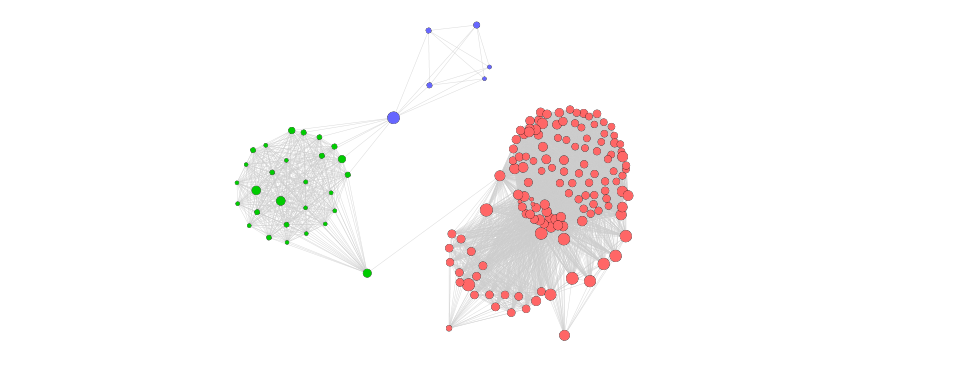
\includegraphics[]{nt_view.png}
\caption{{\bf Communities}
The nodes size corresponds to the average connection weight with its neighbors. Bigger nodes have higher genetic distance with its neighbors.}
\label{fig:communities}
\end{figure}



sobre o betweenness

da 0 - 102 - 0.34
da 1 - 166 - 0.32
da 2 - 137 - 0.06 (muito menor por a comunidade azul é bem pequena)

altos considerando q o bet médio foi 0.0057



\subsection*{Análise espacial das comunidades}

\section*{Discussion}
Nulla mi mi, venenatis sed ipsum varius, volutpat euismod diam. Proin rutrum vel massa non gravida. Quisque tempor sem et dignissim rutrum. Lorem ipsum dolor sit amet, consectetur adipiscing elit. Morbi at justo vitae nulla elementum commodo eu id massa. In vitae diam ac augue semper tincidunt eu ut eros. Fusce fringilla erat porttitor lectus cursus, vel sagittis arcu lobortis. Aliquam in enim semper, aliquam massa id, cursus neque. Praesent faucibus semper libero.

\subsection*{\lorem\ and \ipsum\ Nunc blandit a tortor.}

CO\textsubscript{2} Maecenas convallis mauris sit amet sem ultrices gravida. Etiam eget sapien nibh. Sed ac ipsum eget enim egestas ullamcorper nec euismod ligula. Curabitur fringilla pulvinar lectus consectetur pellentesque. Quisque augue sem, tincidunt sit amet feugiat eget, ullamcorper sed velit. 

Sed non aliquet felis. Lorem ipsum dolor sit amet, consectetur adipiscing elit. Mauris commodo justo ac dui pretium imperdiet. Sed suscipit iaculis mi at feugiat. Ut neque ipsum, luctus id lacus ut, laoreet scelerisque urna. Phasellus venenatis, tortor nec vestibulum mattis, massa tortor interdum felis, nec pellentesque metus tortor nec nisl. Ut ornare mauris tellus, vel dapibus arcu suscipit sed. Nam condimentum sem eget mollis euismod. Nullam dui urna, gravida venenatis dui et, tincidunt sodales ex. Nunc est dui, sodales sed mauris nec, auctor sagittis leo. Aliquam tincidunt, ex in facilisis elementum, libero lectus luctus est, non vulputate nisl augue at dolor. For more information, see \nameref{S1_Text}.

\section*{Supporting Information}

% Include only the SI item label in the subsection heading. Use the \nameref{label} command to cite SI items in the text.
\subsection*{S1 Video}
\label{S1_Video}
{\bf Bold the first sentence.}  Maecenas convallis mauris sit amet sem ultrices gravida. Etiam eget sapien nibh. Sed ac ipsum eget enim egestas ullamcorper nec euismod ligula. Curabitur fringilla pulvinar lectus consectetur pellentesque.

\subsection*{S1 Text}
\label{S1_Text}
{\bf Lorem Ipsum.} Maecenas convallis mauris sit amet sem ultrices gravida. Etiam eget sapien nibh. Sed ac ipsum eget enim egestas ullamcorper nec euismod ligula. Curabitur fringilla pulvinar lectus consectetur pellentesque.

\subsection*{S1 Fig}
\label{S1_Fig}
{\bf Lorem Ipsum.} Maecenas convallis mauris sit amet sem ultrices gravida. Etiam eget sapien nibh. Sed ac ipsum eget enim egestas ullamcorper nec euismod ligula. Curabitur fringilla pulvinar lectus consectetur pellentesque.

\subsection*{S2 Fig}
\label{S2_Fig}
{\bf Lorem Ipsum.} Maecenas convallis mauris sit amet sem ultrices gravida. Etiam eget sapien nibh. Sed ac ipsum eget enim egestas ullamcorper nec euismod ligula. Curabitur fringilla pulvinar lectus consectetur pellentesque.

\subsection*{S1 Table}
\label{S1_Table}
{\bf Lorem Ipsum.} Maecenas convallis mauris sit amet sem ultrices gravida. Etiam eget sapien nibh. Sed ac ipsum eget enim egestas ullamcorper nec euismod ligula. Curabitur fringilla pulvinar lectus consectetur pellentesque.

\section*{Acknowledgments}
Cras egestas velit mauris, eu mollis turpis pellentesque sit amet. Interdum et malesuada fames ac ante ipsum primis in faucibus. Nam id pretium nisi. Sed ac quam id nisi malesuada congue. Sed interdum aliquet augue, at pellentesque quam rhoncus vitae.

\nolinenumbers

%\section*{References}
% Either type in your references using
% \begin{thebibliography}{}
% \bibitem{}
% Text
% \end{thebibliography}
%
% OR
%
% Compile your BiBTeX database using our plos2015.bst
% style file and paste the contents of your .bbl file
% here.
% 
%\begin{thebibliography}{10}
%\bibitem{bib1}
%Devaraju P, Gulati R, Antony PT, Mithun CB, Negi VS. Susceptibility to SLE in South Indian Tamils may be influenced by genetic selection pressure on TLR2 and TLR9 genes. Mol Immunol. 2014 Nov 22. pii: S0161-5890(14)00313-7. doi: 10.1016/j.molimm.2014.11.005

%\bibitem{bib2}
%Huynen MMTE, Martens P, Hilderlink HBM. The health impacts of globalisation: a conceptual framework. Global Health. 2005;1: 14. Available: http://www.globalizationandhealth.com/content/1/1/14.

%\end{thebibliography}


\printbibliography



\end{document}

